\documentclass[letterpaper,10pt]{article}
\usepackage{fullpage}
\usepackage{amsmath}
\usepackage{amssymb}
\usepackage{color}
%\usepackage{fancyhdr}
%\usepackage{graphicx}
\usepackage{tikz}
\usetikzlibrary{mindmap} %for mindmap
\pagestyle{empty}    %takes away pagenumbering
\newcommand\N{\ensuremath{\mathbb N}}
\newcommand\R{\ensuremath{\mathbb R}}
\newcommand\T{\ensuremath{\mathcal T}}
\newcommand\Red[1]{\textcolor{red}{\bf #1}}
\newcommand\Blue[1]{\textcolor{blue}{\bf #1}}
\newcommand\Black[1]{\textcolor{black}{#1}}
%\fancyfoot{}  %to take away pagenumbering
%\oddsidemargin 0.0in 
%\evensidemargin 1.0in 
%\textwidth 6.0in 
\headheight 0in 
\topmargin 0in 
%\textheight 9.0in 
\begin{document}
\begin{center}
%\includegraphics{}
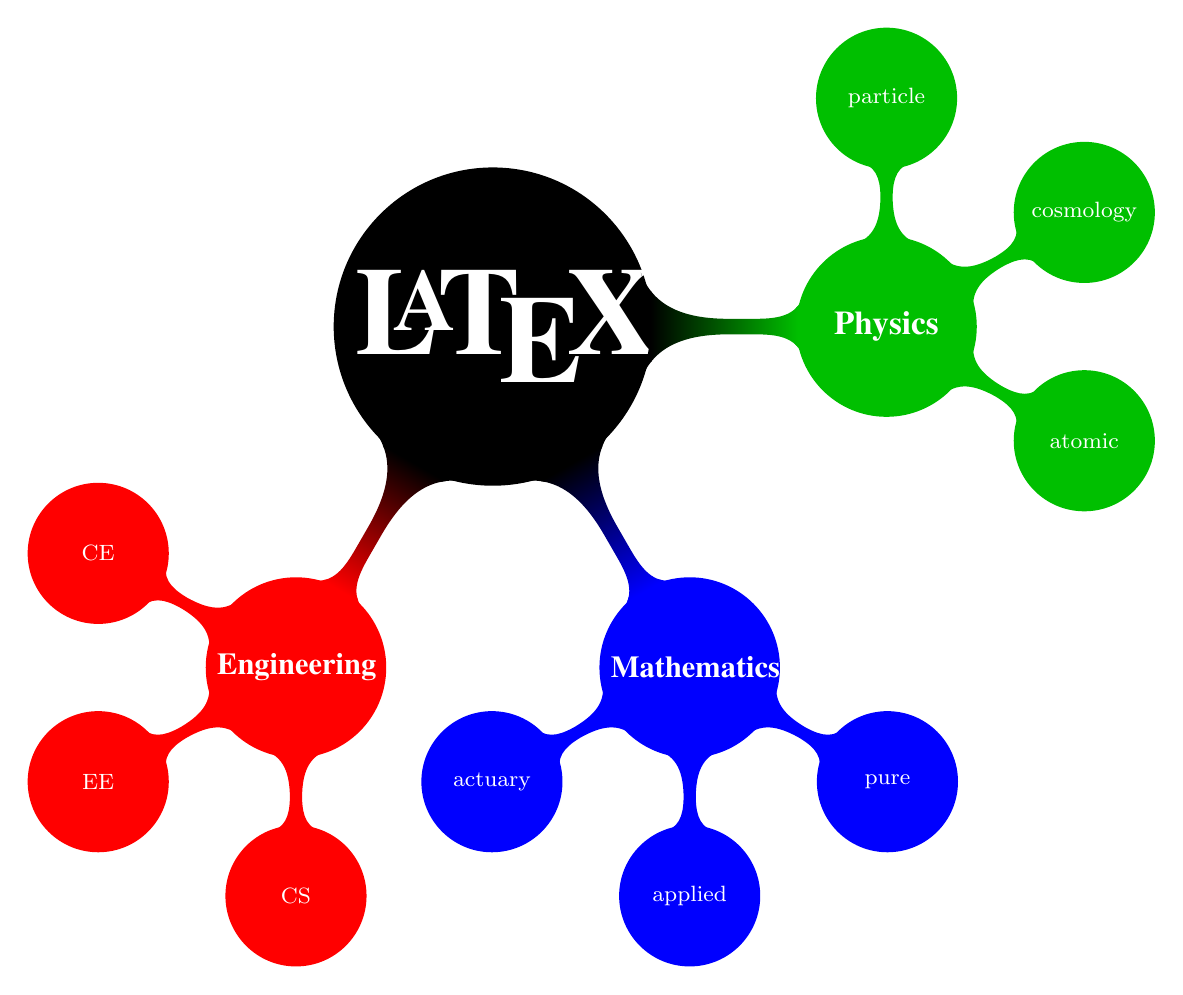
\begin{tikzpicture}
	\path[mindmap, concept color=black, text=white]
	   node[concept] {\fontfamily{ptm}\fontsize{45}{45}\bfseries\selectfont \LaTeX}
	   [clockwise from=0]
	   	child[concept color=green!75!black] {
	   		node[concept] {\fontfamily{ptm}\fontsize{12}{12}\bfseries\selectfont Physics}
			[clockwise from=90]
				child { node[concept] {particle} }
				child { node[concept] {cosmology} }
				child { node[concept] {atomic} }
		}
	   	child[concept color=blue] {
			node[concept] {\fontfamily{ptm}\fontsize{11}{11}\bfseries\selectfont Mathematics}
			[clockwise from=-30]
				child { node[concept] {pure} }
				child { node[concept] {applied} }
				child { node[concept] {actuary} }
		}
		child[concept color=red] {
			node[concept] {\fontfamily{ptm}\fontsize{11}{11}\bfseries\selectfont Engineering}
			[clockwise from=-90]
				child { node[concept] {CS} }
				child { node[concept] {EE} }
				child { node[concept] {CE} }
		};
%\node (a) at (1,1) [circle, draw] {\large {\LaTeX tutorial}};
\end{tikzpicture}
~\\
~\\
{\huge {\bf Want to learn how to create this in \LaTeX ?\\
Take the first step and come to the tutorial. }}
\center
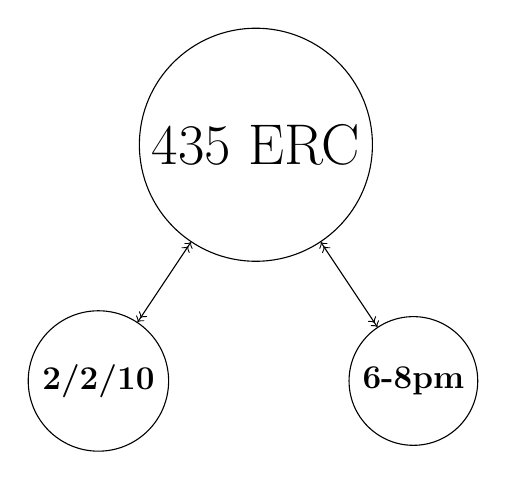
\begin{tikzpicture}
	\node (a) at (0,0) [circle, draw] {\huge 435 ERC};
	\node (b) at (-2,-3) [circle, draw] {\large \bf 2/2/10} 	edge[<<->>](a);
	\node (c) at (2,-3) [circle, draw] {\large \bf 6-8pm}	edge[<<->>](a);
\end{tikzpicture}
~\\
Brought to you by UC's chapter of {\bf \emph{ ACM }}
\\
\includegraphics[scale=0.3]{acm.jpg}



\end{center}
\end{document}